% This is samplepaper.tex, a sample chapter demonstrating the
% LLNCS macro package for Springer Computer Science proceedings;
% Version 2.20 of 2017/10/04
%
\documentclass[runningheads]{llncs}
%
\usepackage{amsmath}
\usepackage{amssymb} % for \therefore
\usepackage{graphicx}
\usepackage{array} % for table cell centering
% Used for displaying a sample figure. If possible, figure files should
% be included in EPS format.
%
% If you use the hyperref package, please uncomment the following line
% to display URLs in blue roman font according to Springer's eBook style:
% \renewcommand\UrlFont{\color{blue}\rmfamily}

\begin{document}
%
\title{An Evaluation of Uninformed and Informed Search Algorithms on the $k$-puzzle Problem}
\subtitle{AY19/20 Semester 2 CS3243 Project 1, Group 37}
%
\titlerunning{Search Algorithms on the $k$-puzzle Problem}
% If the paper title is too long for the running head, you can set
% an abbreviated paper title here
%
\author{Lim Fong Yuan \and
Zhuang Xinjie \and
Otto Alexander Sutianto \and
Mario Lorenzo}
%
\authorrunning{Lim et al.}
% First names are abbreviated in the running head.
% If there are more than two authors, 'et al.' is used.
%
\institute{School of Computing, National University of Singapore% \and
%Springer Heidelberg, Tiergartenstr. 17, 69121 Heidelberg, Germany
%\email{lncs@springer.com}\\
%\url{http://www.springer.com/gp/computer-science/lncs} \and
%ABC Institute, Rupert-Karls-University Heidelberg, Heidelberg, Germany\\
%\email{\{abc,lncs\}@uni-heidelberg.de}
}
%
\maketitle              % typeset the header of the contribution
%
%\begin{abstract}
%The abstract should briefly summarize the contents of the paper in
%150--250 words.

%\keywords{First keyword  \and Second keyword \and Another keyword.}
%\end{abstract}
%
%
%
\section{Problem Specification}
%\begin{enumerate}
%\item A suitable representation should be specified to define the problem
%\item It should facilitate the formulation of search-based solutions
%\end{enumerate}

Fix $n \in \bbbz_{\geq 2}$. Let $k = n^2 -1$.
A valid state $v$ is a $n \times n$ array with the entries $v_{(x,y)}$ containing a permutation of the integers $[0,k]$. $V$ is the set of valid states.
Each valid state has a unique coordinate $e = (x_e,y_e)$ such that $v_e = 0$. Call $v_e$ the empty cell of $v$.
An initial state $s$ is a valid state with $e = (n,n)$.
The goal state $g$ is where $g_{(x,y)} = (x-1)n+y$ for all $(x,y) \in (\bbbz_{[1,n]})^2$, except for $g_{(n,n)}$ which is $0$.
Let $A = \{\texttt{up}=(-1,0),\texttt{down}=(1,0),\texttt{left}=(0,-1),\texttt{right}=(0,1)\}$ be the set of actions.
The transition function $T: V \times A \to V$ is where $T(v,a) = v'$ with $v'$ being identical to $v$ except with $(v'_{e-a},v'_e) = (v_e,v_{e-a})$.% (Invalid output states are rejected.)

The problem is to determine if $g$ is reachable from a given initial state $s$, and if so, specify a sequence of actions $p \in A^\ast$ that leads from $s$ to $g$.



%Please try to avoid rasterized images for line-art diagrams and schemas. Whenever possible, use vector graphics instead (see Fig.~\ref{fig1}).
\begin{figure}
	\centering
	%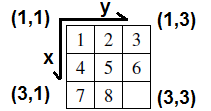
\includegraphics[width=\textwidth]{coord_system.png}
	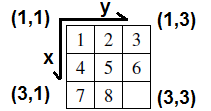
\includegraphics{coord_system.png}
	\caption{The coordinate system on the goal state, in the case of $n=3$.} \label{fig:coordsystem}
\end{figure}



\section{Technical Analysis}
All the evaluated algorithms initially check for the solvability of the given puzzle, using the criterion that was proposed and proved in \cite{Solvability}. This is to guarantee to the search algorithms that the goal state is reachable, so they do not need to exhaust an extremely large solution space.
The criterion is restated and reproved in Appendix \ref{subsec:solvability}.

\subsection{[...] Search (xxS) (Uninformed)}
\subsubsection{Correctness}
[BLAH]

\subsubsection{Efficiency}
Given any valid state, there are up to $|A|=4$ possible actions. However, the initial state only has 2 possible actions, and every state thereafter has an action that backtracks and can thus be discounted, thus the maximum branching factor $b$ of the problem space is $|A|-1=3$. // This algorithm thus has $O(3^d)$ time and $O(3^d)$ space complexity.

\subsection{A* Search (Informed)}
\subsubsection{Correctness}
[BLAH]

\subsubsection{Efficiency}
[BLAH]

\subsubsection{Heuristics}
In this subsection, let $v$ be any (valid) state and $v'$ be any state reachable from $v$ by a single (valid) action. Their difference is the position of a single tile $T$ (the empty cell is not counted), which has swapped placed with the empty cell which it is adjacent to. Their absolute difference in cost $d(v,v') = 1$. Let $d_h(v,v') := h_1(v')-h_1(v)$ be their difference in heuristic cost.

\paragraph{$h_1$: Sum of Manhattan distances of each (non-empty) tile from its final position.}
Proof of consistency: $T$ is moved either closer to ($d_{h_1} = -1$) or farther away from ($d_{h_1} = 1$) its final position by a Manhattan distance of 1.
In any case, $|d_{h_1}(v,v')|\leq 1 \implies h_1(v) \leq 1+h_1(v') = d(v,v')+h_1(v')$, $\therefore$ $h_1$ is consistent. $\qed$

\paragraph{$h_2$: Number of misplaced (non-empty) tiles.}
Proof of consistency: $T$ is either placed on ($d_{h_2} = -1$), moved out of ($d_{h_2} = 1$), or remains away ($d_{h_2} = 0$) from its final position.
In any case, $|d_{h_2}(v,v')|\leq 1 \implies h_2(v) \leq 1+h_2(v') = d(v,v')+h_2(v')$, $\therefore$ $h_2$ is consistent. $\qed$

\paragraph{$h_3$: Heu3}
The 3 heuristics should be distinct and non-trivial; for example, your heuristic should not be a constant, a simple linear transformation of other heuristics, or any simple function of another heuristic like a square root of another

Consistency/Admissibility: Your heuristic must be provably admissible, or (preferably) consistent. In either case you must formally prove this property. Note that consistency implies admissibility but not the other way around. Thus, if you show admissibility, you should provide a (preferably simple) counterexample where your heuristic violates consistency.



\section{Experimental Setup}
The performances of the uninformed search and the informed search with each of the three heuristics have been experimentally measured, and consolidated in Table \ref{tab:results}. The inputs used draw from a specified subset of valid initial states, under a uniform random distribution, and the average results from 200 inputs were taken for each experiment. The metrics used to evaluate each algorithm are the absolute time taken to execute the algorithm, and the number of nodes seen. These metrics directly reflect the time and memory requirements of each algorithm respectively.

The algorithms were coded in Python 3.x.x and the experiments were run on a [OS] machine with a [processor] and 16 GB of RAM. Absolute time was measured with \texttt{[Python time library]}.

% If there was a more lax report length requirement, it could be neater to split this into a time table and #nodes table
\begin{table}[h]\label{tab:results}
\centering
\caption{Experiment results.}
\begin{tabular}{|c|
		>{\centering}p{0.105\textwidth}|>{\centering}p{0.095\textwidth}|
		>{\centering}p{0.105\textwidth}|>{\centering}p{0.095\textwidth}|
		>{\centering}p{0.105\textwidth}|>{\centering}p{0.095\textwidth}|
		>{\centering}p{0.105\textwidth}|>{\centering\arraybackslash}p{0.095\textwidth}|} % compile error without \arraybackslash for some reason
\hline
      & \multicolumn{2}{c|}{xxS} & \multicolumn{2}{c|}{A* with $h_1$} & \multicolumn{2}{c|}{A* with $h_2$} & \multicolumn{2}{c|}{A* with $h_3$} \\
\hline
Inputs & Time taken (s) & \#Nodes seen & Time taken (s) & \#Nodes seen & Time taken (s) & \#Nodes seen & Time taken (s) & \#Nodes seen \\
\hline
3x3 Solvable   & 1 & 1 & 1 & 1 & 1 & 1 & 1 & 1 \\
3x3 All        & 1 & 1 & 1 & 1 & 1 & 1 & 1 & 1 \\
\hline
4x4 Solvable   & 1 & 1 & 1 & 1 & 1 & 1 & 1 & 1 \\
4x4 All        & 1 & 1 & 1 & 1 & 1 & 1 & 1 & 1 \\
\hline
5x5 Solvable   & 1 & 1 & 1 & 1 & 1 & 1 & 1 & 1 \\
5x5 All        & 1 & 1 & 1 & 1 & 1 & 1 & 1 & 1 \\
5x5 Unsolvable & 1 & 1 & 1 & 1 & 1 & 1 & 1 & 1 \\
\hline
\end{tabular}
\end{table}



\section{Results and Discussion}
As Table \ref{tab:results} shows, [A* with $h_1$ is better than DFS].
This agrees with our theoretical analysis.



\pagebreak
\appendix
\section{Appendix: Proofs}
\label{app:proofs}
%\noindent Displayed equations are centered and set on a separate line.
%\begin{equation}
%x + y = z
%\end{equation}

% the environments 'definition', 'lemma', 'proposition', 'corollary',
% 'remark', and 'example' are defined in the LLNCS documentclass as well.
\subsection{Solvability of an Initial State \cite{Solvability}}
\label{subsec:solvability}
\begin{lemma}\label{lem:evennumofvertactions}
It always takes an even number of vertical actions to get from any (solvable) initial state $s$ to the goal state $g$ (or equivalently, from $g$ to $s$).
\end{lemma}
\begin{proof}
Colour the board black and white in alternating rows, with the bottom row coloured white. On every vertical action, the empty cell either moves from a white row to a black row, or from a black row to a white row. The empty cell starts on a white row and ends on a white row, which requires an even number of vertical actions. $\qed$
\end{proof}

\begin{definition}\label{def:inversion}
For any given state $v$, write out its entries in a sequence $S(v)$, ignoring the empty cell. i.e. $S(v)_i = v_{(\lceil i/n\rceil, ((i-1) \mod n) +1)}$ for $i \in \bbbz_{[1,n^2]}$, then remove the empty cell from $S(v)$ (so it is now indexed from $1$ to $k$). An \textbf{inversion} is a pair of indices $(i,j)$ such that $i < j$, but $S(v)_i > S(v)_j$.
\end{definition}
Every state $v$ has a well-defined number of distinct inversions, denote it $I(v)$. $I(v)$ can be calculated by tallying how many distinct pairs in $v$ are inversions, which takes $O(k^2)$ time as there are $^kC_2 = \frac{k(k+1)}{2}$ pairs to check.

\begin{theorem}\label{thm:solvability}
An initial state $s$ is solvable if and only if $I(s)$ is even.
\end{theorem}
\paragraph{$(\implies)$}
A solvable state is one that can reach the goal state $g$ in a finite number of actions. Since each action is reversible by an opposite action, this can be restated as: A state is solvable if and only if it is reachable from $g$ in a finite number of actions.

Now given a solvable initial state $s$, consider a sequence of actions taken to move from $g$ to $s$, and how $I(v)$ changes across it. For each action, consider its start state $v$ and result state $v'$. If an action moves horizontally, $S(v) = S(v')$, thus $I(v') = I(v)$.

If an action moves vertically, then $n-1$ swaps between adjacent elements occur from $S(v)$ to $S(v')$, and each swap either introduces or resolves an inversion, which flips the parity of $I(v')$. If $n$ is odd, then the number of swaps $n-1$ is even and thus the parity of $I(v')$ is always the same as $I(v)$. If $n$ is even, then $n-1$ is odd and thus the parity of $I(v')$ is always different from $I(v)$.

It has thus been shown that the parity of $I(v)$ flips only when $n$ is even and a vertical action is taken. Even then, by Lemma \ref{lem:evennumofvertactions}, there are an even number of vertical actions, and thus the parity of $I(v)$ flips an even number of times over the entire path from $g$ to $s$. Therefore, $I(s)$ has the same parity as $I(g)$. And $I(g) = 0$ is even.
$\qed$

\paragraph{$(\impliedby)$}
This is essentially a tedious proof by construction, and the proof is deferred. The general strategy is to move 1 to the right place and never move it again, then do the same with 2, then 3, and so on, up until the puzzle is solved.
$\qed$



%Multiple citations: \cite{ref_article1,ref_book1,ref_proc1,ref_url1}

% ---- Bibliography ----
% BibTeX users should specify bibliography style 'splncs04'.
% References will then be sorted and formatted in the correct style.
\bibliographystyle{splncs04}
\bibliography{mybib}

\end{document}
